\section{Background and Related Work}

\subsection{Prior work in the literature}
Robots have the potential to help distribute expertise around long distances using tele-robotics, to reduce costs by automating routine tasks, and protect workers against occupational hazards and ergonomic strain.  These potential benefits are already being adopted into healthcare.

\textcolor{red}{TODO: need references on gender and age bias with technology.  Needed from Jeanine}

\textcolor{red}{TODO: need references on economic impact of robotics and automation.  Needed from Alex}

\textcolor{red}{TODO: clean up and add references to telerobotics and autonomy}
Collaboration between humans and autonomous robotic agents has the potential to improve safety and efficiency across a wide range of industrial settings, including manufacturing, medicine, maintenance, and construction (Fong, Thorpe, \& Baur, 2001; Tan, Duan, Zhang, Kato, \& Arai, 2009; Kock, et al., 2011; McDonald, Small, Graves, \& Cannon, 1997). An important set of challenges in the design and implementation of human-autonomy collaborative systems is developing a clear understanding of the task environment and potential agent roles, the interdependencies between human and robotic agents, and the impact of disruptions (e.g. (Tan, Duan, Kato, \& Arai, 2010; Hoffman \& Breazeal, 2004; Drury, Scholtz, \& Yanco, 2003; Mutlu, Osman, Forlizzi, Hodgins, \& Kiesler, 2006)).

Managing the safety and efficiency of such systems under dynamic settings is particularly challenging given the complexities of such work environments. For example, a response to a dynamic failure (such as a human or robot breakdown) will have different considerations dependent upon the work architecture (the functional allocation between robots and human) and nature of the work environment (structured vs. unstructured, e.g. (Kolski, Ferguson, Bellino, \& Siegwart, 2006; Scholtz, 2003)). How to effectively optimize safety and efficiency, which are often competing variables, and dynamically reallocate resources accordingly creates a challenging problem for managers and schedulers of such complex systems.

Management of worker and equipment scheduling, coordinating equipment maintenance, tracking of production and safety metrics and ensuring appropriate quality control are all key considerations for supervisors of modern manufacturing environments (e.g. (Brumson, 2008; Brandimarte, 1999)). The challenges associated with managing all of these factors are made more complex by the introduction of collaborative human and robotic work environments, which is a nascent interdisciplinary field. In current manufacturing environments humans and robots work in zones of exclusivity, both physically and for task assignments (Krüger, Lien, \& Verl, 2009; Fryman, 2014; Unhelkar \& Shah, 2015). However, with the emergence of robots that can work alongside humans, like the Baxter™ robot (Figure 1), soon human-robot teams  that jointly work on tasks will be commonplace. 

The increased capabilities that collaborative human-robot teams will bring also introduce complexities in scheduling activities, particularly under dynamic replanning conditions  that occur when both humans and robots “malfunction”, i.e., humans call in sick at the last minute or robots unexpectedly stop working (Wilcox, Nikolaidis, \& Shah, 2013; Stubbs, Wettergreen, \& Hinds, 2007). The impact of these contingencies on the productivity of a manufacturing line will depend upon the nature of the task, the architecture of the work environment, and the availability of substitute workers (either human or robot). The flexibility of the work architecture will dictate the options with which a scheduler or manager can shift assets to minimize the impact on production when problems arise. Indeed, even in current manufacturing operations, such last-minute, dynamic replanning scenarios are difficult to manage even without the added complexity of jointly-tasked human-robot teams (Leitão \& Restivo, 2008). In collaborative human-autonomy environments, addressing such dynamic replanning conditions will be even more challenging, and an inefficient decision could result in a significant decrement in production or increase in safety risk.

There is a long history of research on the incorporation of robotic agents in manufacturing systems (Hägele, Nilsson, \& Pires, 2008; Krüger, Lien, \& Verl, 2009). Typically, these efforts have focused on the use of physical or temporal separation from humans to ensure safety (Marvel \& Bostelman, 2013; Fryman, 2014; Unhelkar \& Shah, 2015; Tan, Duan, Zhang, Kato, \& Arai, 2009; Eilering, Franchi, \& Hauser, 2014). More recently, there has been interest in the inclusion of robotic systems in manufacturing environments that require close interaction and collaboration of human and robotic agents (Office of the Secretary of Defense, 2013; Ryan \& Cummings, 2014; Scanlon, 2009; Rio Tinto, 2014) (Nikolaidis, Ramakrishnan, Gu, \& Shah, 2015). Most of the prior research on human-robot collaboration has focused on the localized methods of interaction and communication of commands and intent between a human worker and a robotic worker (Gombolay, Huang, \& Shah, 2015; Inagaki, Sugie, Aisu, Ono, \& Unemi, 1995; Green, 2008; Bauer, Wollherr, \& Buss, 2008; Fernandez, Balaguer, Blanco, \& Salichs, 2001; Li \& Hauser, 2015; Hoffman, 2013). For example, Fernandez et al. (2001) experimented with determining intent of humans in a collaborative carrying task based on the force signal measured in the arm gripper. Maintaining safety in such collaborative environments has also continued to be an active area of research (Tan \& Arai, 2011; Fryman, 2014; Pedrocchi, Vicentini, Matteo, \& Tosatti, 2013; Matthias, et al., 2011). However, there is very little research on more global interactions of humans and robots in terms of developing integrated schedules, and how such interactions drive large productivity and safety goals.

Traditionally, scheduling of robotic systems have focused on artificial intelligence (AI) or rule-based scheduling (e.g. (Miyashita, 1998; Hall, Kamoun, \& Sriskandarajah, 1998; Sikora \& Shaw, 1997)), though have acknowledged the usefulness of including a human supervisor in the scheduling process (Chen \& Guerrero, 1992). It has been demonstrated that human supervisors can improve scheduling decision-making through the coaching of automated systems, e.g. (Barnes, Chen, Jentsch, \& Redden, 2011; Cummings, Brzezinski, \& Lee, 2007; Adams, 2009; Chen \& Barnes, 2012; Fagerholt, 2004; Törnquist, 2006). While these studies have shown the benefit of automation-aided decision making, these environments generally considered automation in terms of “expert” systems, which operate deterministically by pre-programmed rules. What they have not addressed is the task dependencies and scheduling challenges associated with proposed human-autonomy collaborative manufacturing environments, which contain significant uncertainty and many more stochastic variables.

Still a relatively new field, current research into task scheduling for robotic and collaborative environments focuses on detailed elements of timing and motion constraints (e.g. (Gombolay, Wilcox, \& Shah, 2013; Shah, Conrad, \& Williams, 2009; Boerkoel Jr \& Durfee, 2011; Gowal \& Martinoli, 2012), but does not address higher level considerations such as short and long term impacts to higher level global considerations including overall schedule, throughput, maintenance scheduling, and ergonomic risk. The proposed work aims to fill these gaps by investigating decision-support tools for collaborative manufacturing environments that incorporates both short and long term, and local and global implications of current and proposed schedules.


\subsection{Related work of the investigators}

% \begin{wrapfigure}{r}{0.75\linewidth}
\begin{figure}[h!!]
\centering
% \vspace{0.8ex}
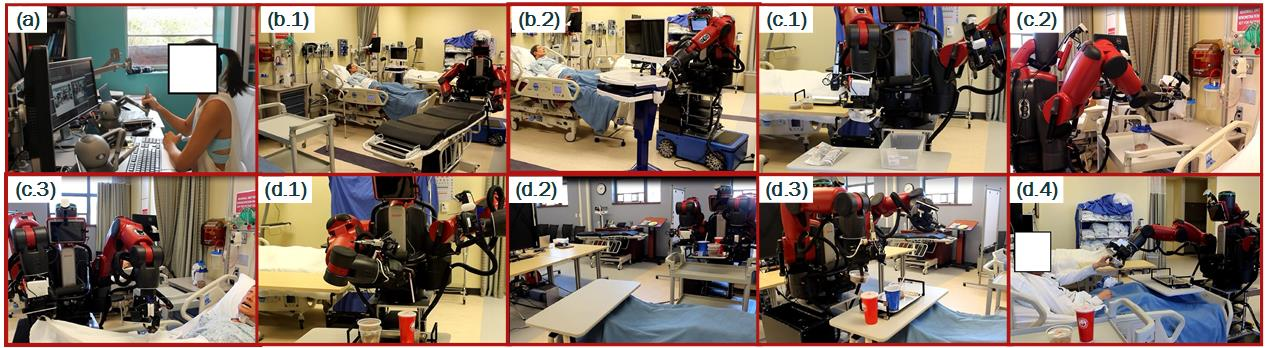
\includegraphics[width=0.99\linewidth]{fig//NursingTask}
\caption{Under (a) direct teleoperation, a mobile humanoid robot tasks can perform complex nursing tasks, including (b.1-2) moving a portable medical devices; (c.1-3) organizing and cleaning the patient's room; and (d.1-4) preparing and serving food to a patient. These tasks involves the coordination among multiple robot components for manipulation, locomotion and active perception.}
\label{Tasks}
\vspace{1ex}
\end{figure}
% \end{wrapfigure}

\begin{itemize}
\item \textbf{Tele-nursing Robots} In response to the outbreak of highly infectious diseases, such as Ebola (2015) and Zika (2016), Tele-Robotic Intelligent Nursing Assistant (TRINA) --- a tele-presence-tele-action mobile humanoid robot system --- has been developed and over frequently performed nursing tasks (see~\fig{Tasks}). The nursing robot is equipped with fixed cameras mounted at the head and chest, and moving cameras attached to the wrists. Thus, a teleoperator is able to control the coordination of the robot's perception and action arms, in addition to the coordination of different robot components (e.g., arms, hands, mobile base). The experimental system evaluation has demonstrated that on average the tele-nursing robotic system controlled by expert teleoperator is 95X slower than expert human nurse. This performance can be significantly improved by developing a teleoperation interface of more transparent perception and motion mapping. 

\zhi{Figures for tele-surgery tasks to be added}

\item \textbf{Tele-surgical Robots} In robot-assisted minimally invasive surgery, a surgeon needs to control the motion of surgical robot arms while adjusting the endoscopic camera to perceive the surgical site. The motion coordination become more complicated when multiple surgical instruments are operating in the shared workspace. The endoscopic camera needs to appropriately with respect to the operating surgical tools, so that the surgeon can intuitively and correctly perceive the spatial relationship at the operation site. The teleoperation interfaces also need to inform the surgeons of their task performance and the patient vital signs, to assist their operation and decision-making. \textcolor{red}{TODO: need details from Jacob.}

The challenges in hospital administration are compounded by significant scheduling uncertainties such as unplanned absences by workers, equipment breakdowns, or worker injuries. The ability of supervisors and management to dynamically adapt role assignments and schedules (what we term as dynamic replanning) is important for dealing with these uncertainties and maintaining adequate patient care. Our prior work has included the preliminary design of a decision support tool for scheduling human shifts in manufacturing environments (Malik, 2013) (Figure 4). This tool allows a supervisor to view the current schedule in the context of required skills and individual ergonomic risk. 

\textcolor{red}{TODO: add prior related work in gender bias, economics, etc.  Needed from Jeanine, Alex}
% \zhi{Figures for tele-rehabilitation tasks to be added}

% \item \textbf{Tele-rehabilitation Robots} Tele-rehabilitation exoskeletons enable therapists to guide and assist remote patients with power augmentation  


\end{itemize}